\documentclass{article}
\usepackage[colorlinks=true, allcolors=blue]{hyperref}
\usepackage{tabularray}
\usepackage{amssymb}
\usepackage{graphicx} % Required for inserting images

\title{Results}
\author{Automatic Project Detection And Tooling For Devs}
\date{}

\begin{document}
\maketitle

\clearpage

During the project with the Automatic Project Detection and Tooling for Devs team, the primary goal was to create a program that simplifies the process of running executable files for developers. The tool is designed to automatically detect all runnable scripts and executables within the given working directory. It not only identifies these files but also provides an intuitive interface for executing them with ease. Users can supply the necessary arguments directly through the tool, ensuring seamless and efficient script execution. This innovation significantly streamlines the workflow, saving developers time and effort while improving overall productivity.

\section{Marketing}

We have created a marketing poster with the team, showcasing the main pages of our software. Alongside this, we also produced a video that highlights the key features and demonstrates how to use them effectively. Both the poster and the video aim to provide a clear and engaging overview of our software, helping potential Users to understand its capabilities and benefits.

\subsection{Marketing poster}
The poster is available on \href{https://github.com/CsullogBeni/szofttech/blob/main/documentation/img/poster.png}{github},
\begin{figure}[h]
    \centering
    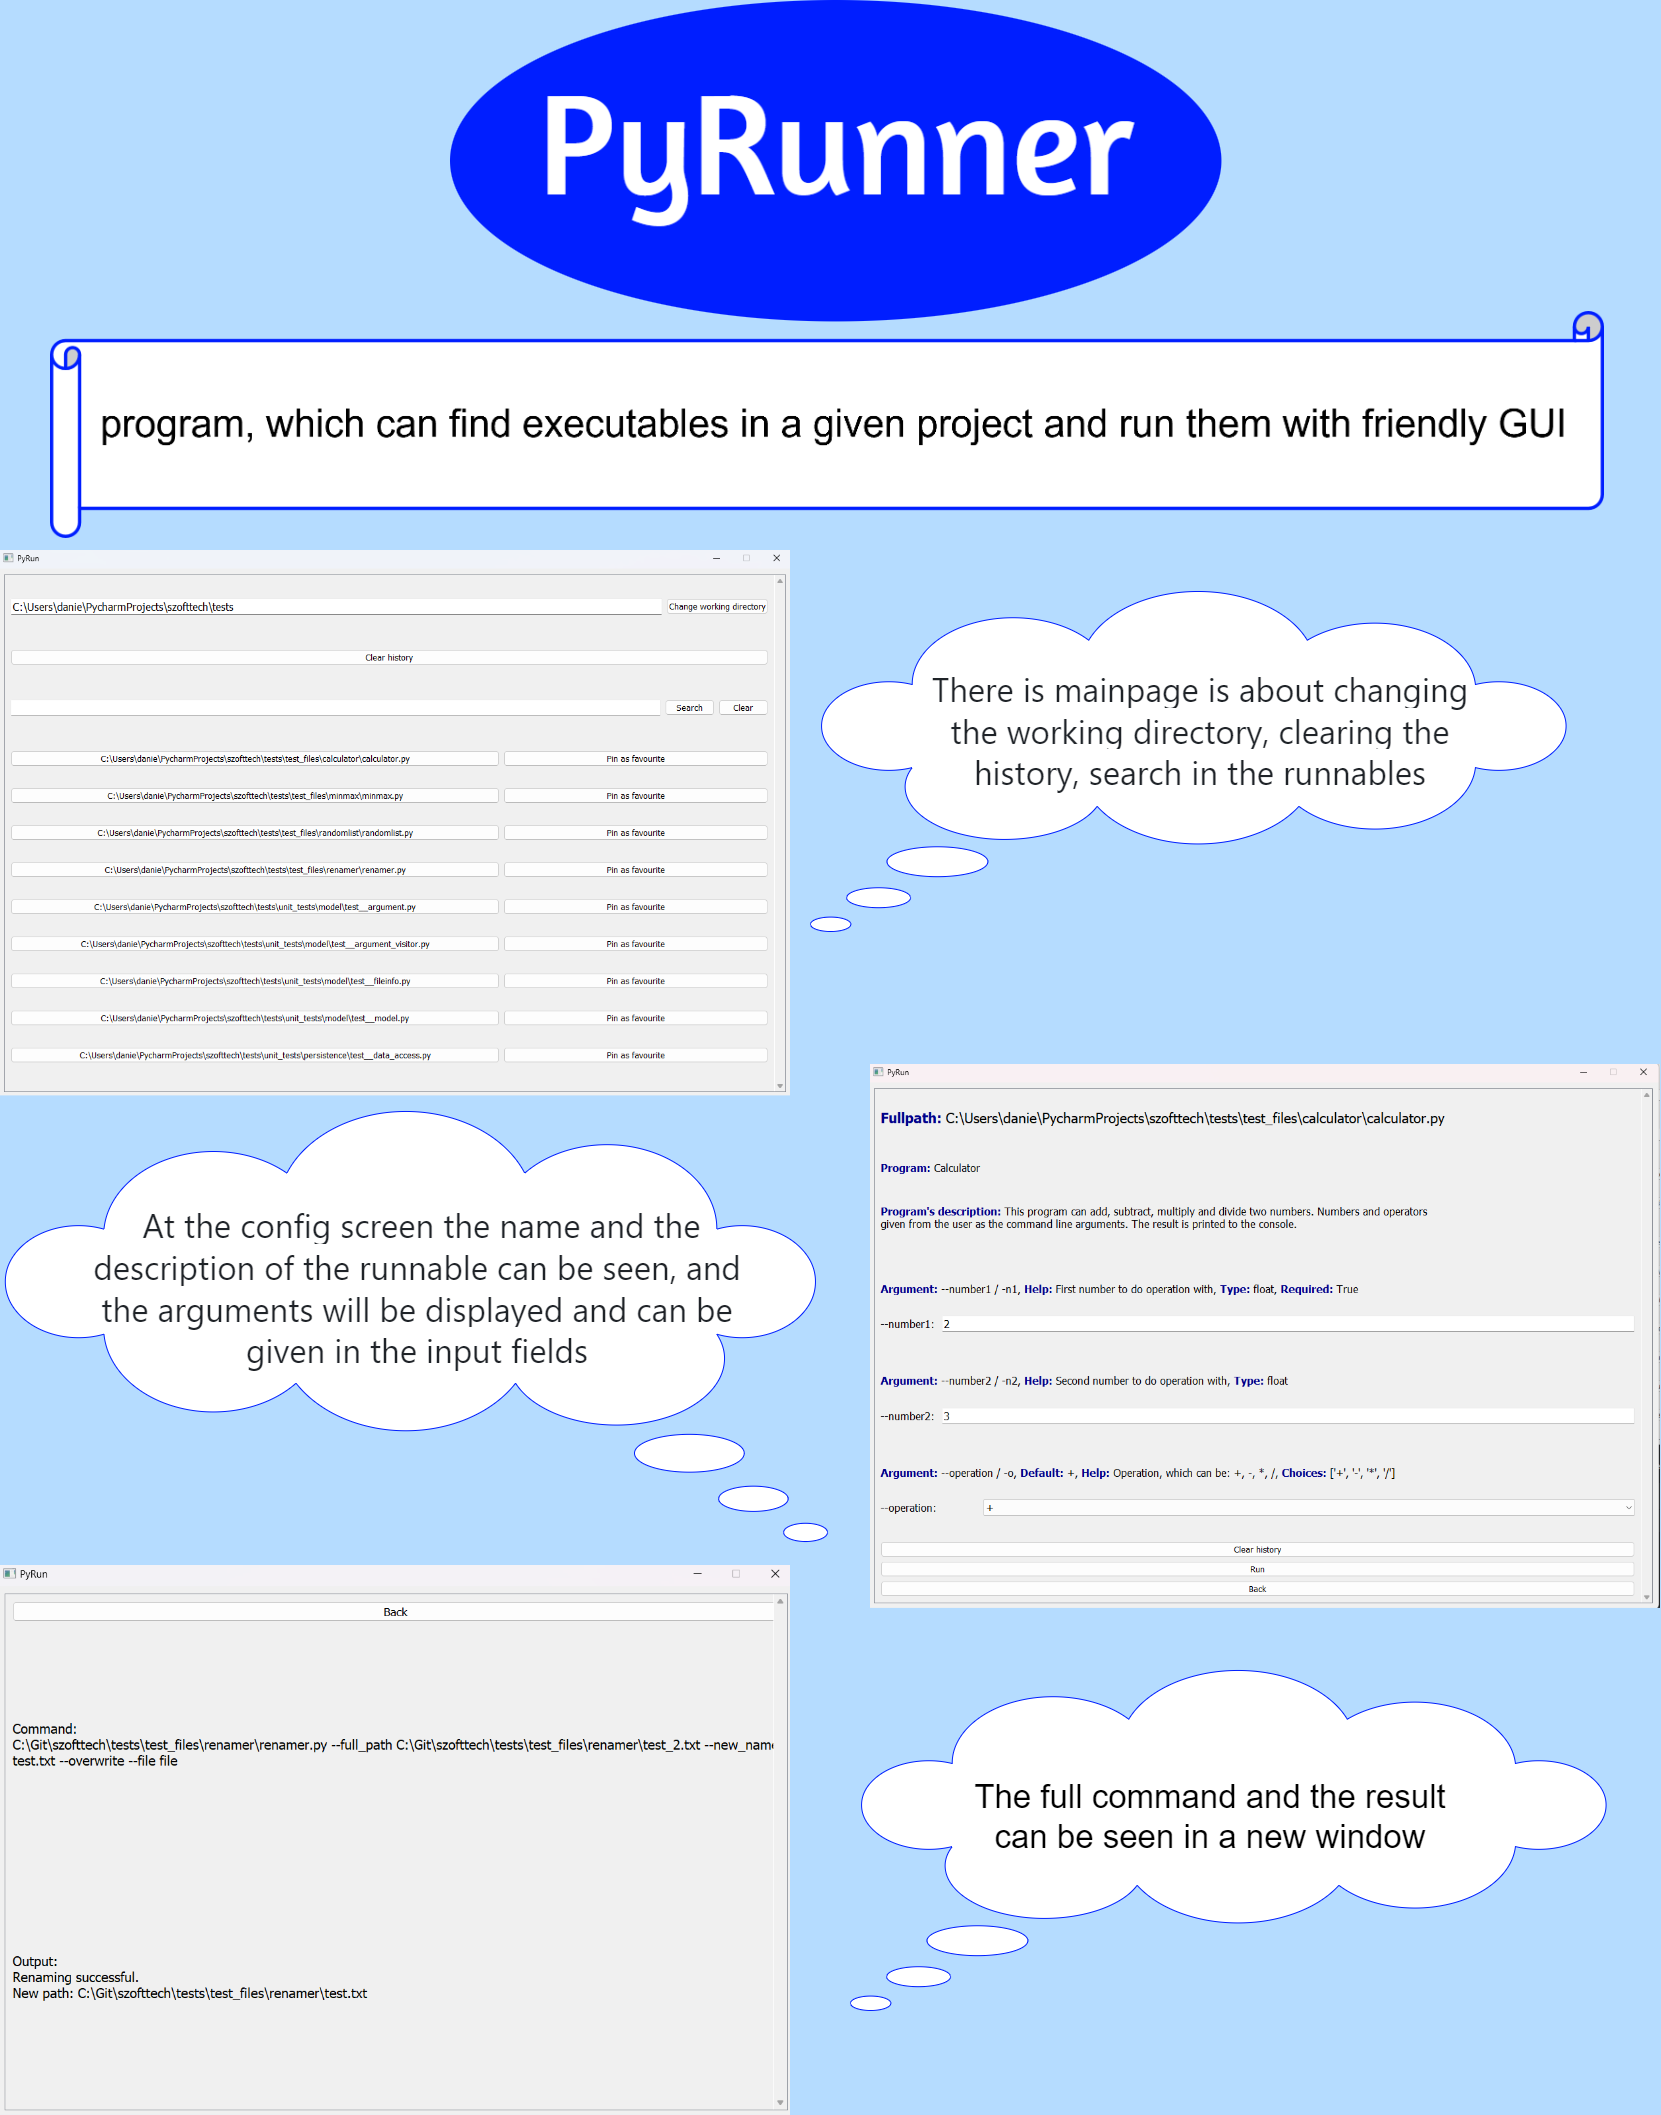
\includegraphics[width=0.8\linewidth]{img/poster.png}
    \caption{Marketing poster}
    \label{fig:enter-label}
\end{figure}

\subsection{Marketing video}

The video is available on \href{https://github.com/CsullogBeni/szofttech/tree/main/documentation/video}{github}.

\subsection{Software requirements}

The following tools and environments are required:

\begin{itemize}
    \item Operating System\@: Windows/Linux/MacOS
    \item Programming Language\@: Node.js or Python (v3.8+)
    \item Additional dependencies\@: PyQt5
    \item Disk space\@: At least 500MB of free space
    \item RAM\@: 4GB minimum (recommended 8GB for better performance)
\end{itemize}

\section{Software installation}

To install the software, follow these steps:

\begin{enumerate}
    \item Open a command line prompt, where you want to install your software
    \item Clone the repository\@: \texttt{git clone https://github.com/CsullogBeni/szofttech.git}.
    \item Activate conda environment or download Python v3.8 or higher
    \item Install dependencies\@: Run \texttt{pip install PyQt5}
    \item Set python path: \texttt{set PYTHONPATH=<Full path to the directory that contains the project>}
    \item Start the application from a command line prompt. Navigate to the directory that contains the project. Run: \@\texttt{python ./src/view/main.py}.
\end{enumerate}

\section{Project tools}

\subsection{Version Control System}

Throughout the development process, we utilized Git as our version control system and hosted the project on GitHub. The entire project including tasks, pull requests, documentation and a detailed README file is available there. You'll also find various marketing materials, brainstorming notes and ideas shared during the project. This comprehensive repository reflects both the technical and creative efforts behind our work, making it a valuable resource for anyone interested in exploring the project's details.

Useful links to the project:
\begin{itemize}
    \item Github that contains the whole project: \\ \href{https://github.com/CsullogBeni/szofttech}{https://github.com/CsullogBeni/szofttech}
    \item Documentation that contains the User stories, MVP, Plan, Retrospective and results: \\ \href{https://github.com/CsullogBeni/szofttech/tree/main/documentation}{https://github.com/CsullogBeni/szofttech/tree/main/documentation}
    \item Here are all the tasks throughout the project: \\  \href{https://github.com/CsullogBeni/szofttech/issues?q=}{https://github.com/CsullogBeni/szofttech/issues?q=}
    \item All the pull requests that are made: \\ \href{https://github.com/CsullogBeni/szofttech/pulls?q=}{https://github.com/CsullogBeni/szofttech/pulls?q=}
    \item You can find here the directory that contains all the implemented source files: \\ \href{https://github.com/CsullogBeni/szofttech/tree/main/src}{https://github.com/CsullogBeni/szofttech/tree/main/src}
    \item We implemented unit test and system test files for the project: \\ \href{https://github.com/CsullogBeni/szofttech/tree/main/tests/unit_tests}{https://github.com/CsullogBeni/szofttech/tree/main/tests/unit}
    \item Also we have created a code base that contains many runnable scripts, and we have used them to test our program: \\  \href{https://github.com/CsullogBeni/szofttech/tree/main/tests/test_files}{https://github.com/CsullogBeni/szofttech/tree/main/tests/files}
    \item We made a few discussions as well: \\ \href{https://github.com/CsullogBeni/szofttech/discussions}{https://github.com/CsullogBeni/szofttech/discussions}
\end{itemize}

\section{Project team}
    Members:
    \begin{itemize}
        \item Zsófia Laczkó 
        \item Borbála Merth 
        \item Márton Petes
        \item Dániel Gergely 
        \item Benedek Csüllög
    \end{itemize}

\subsection{Zsófia Laczkó}
    \begin{tabular}{@{}p{0.7\textwidth}@{} p{0.2\textwidth}@{}}
    Full stack developer
    
    Main tasks:
    \begin{itemize}
        \item Implementation in Model layer
        \item GUI implementation
    \end{itemize}
    &
    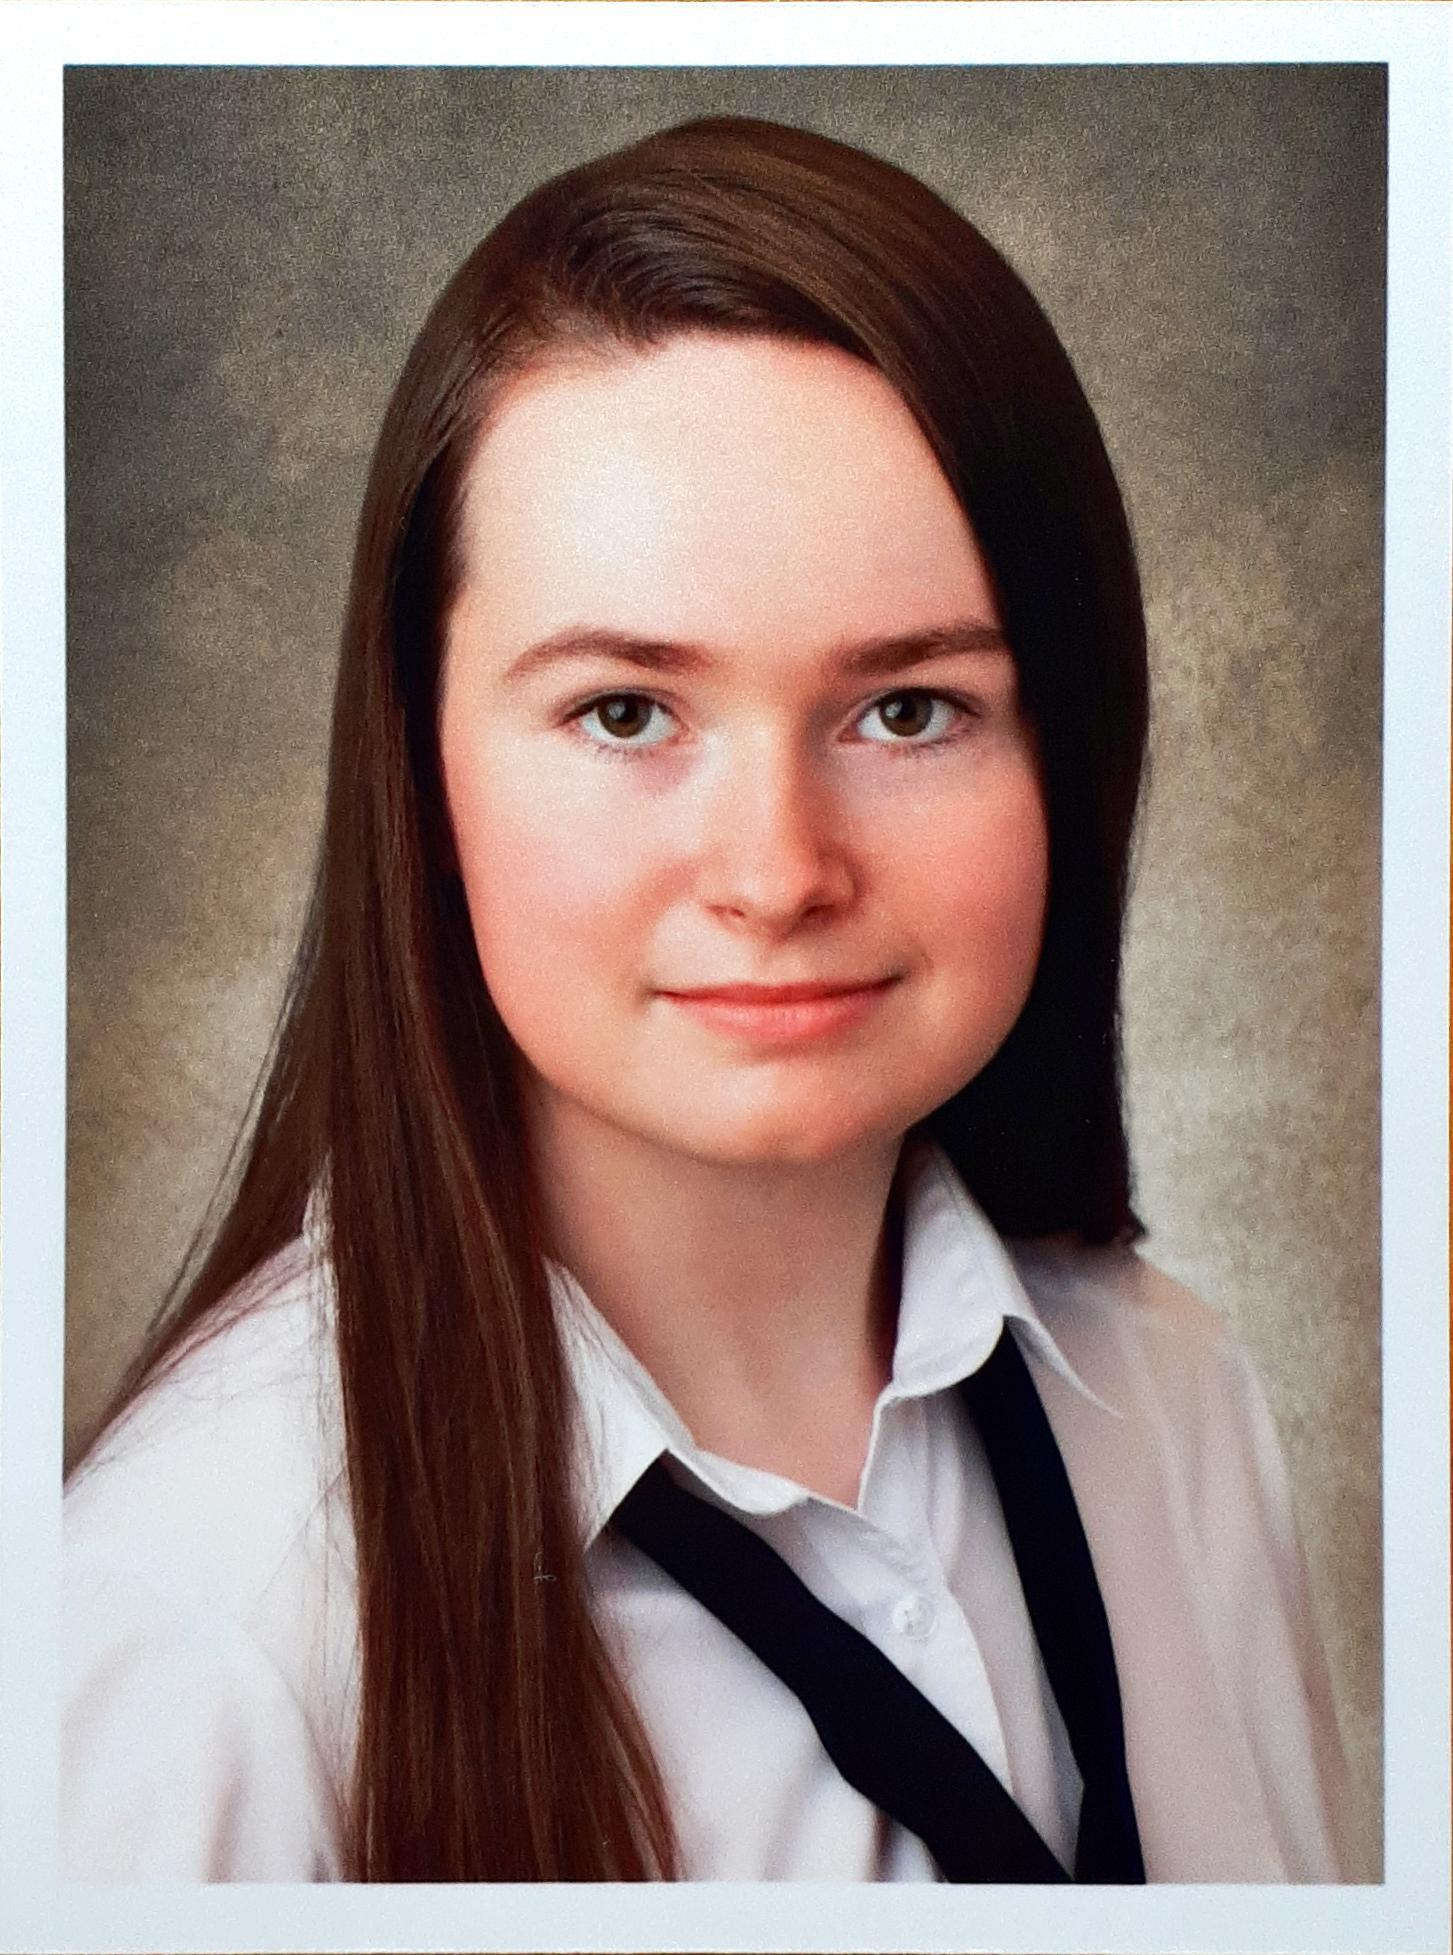
\includegraphics[width=\linewidth]{img/Zsofia_Laczko.jpg}
    \end{tabular}

\subsection{Borbála Merth}
    \begin{tabular}{@{}p{0.7\textwidth}@{} p{0.2\textwidth}@{}}
    Software engineer and architect
    
    Main tasks:
    \begin{itemize}
        \item Architecture of the program
        \item Program documentation
    \end{itemize}
    &
    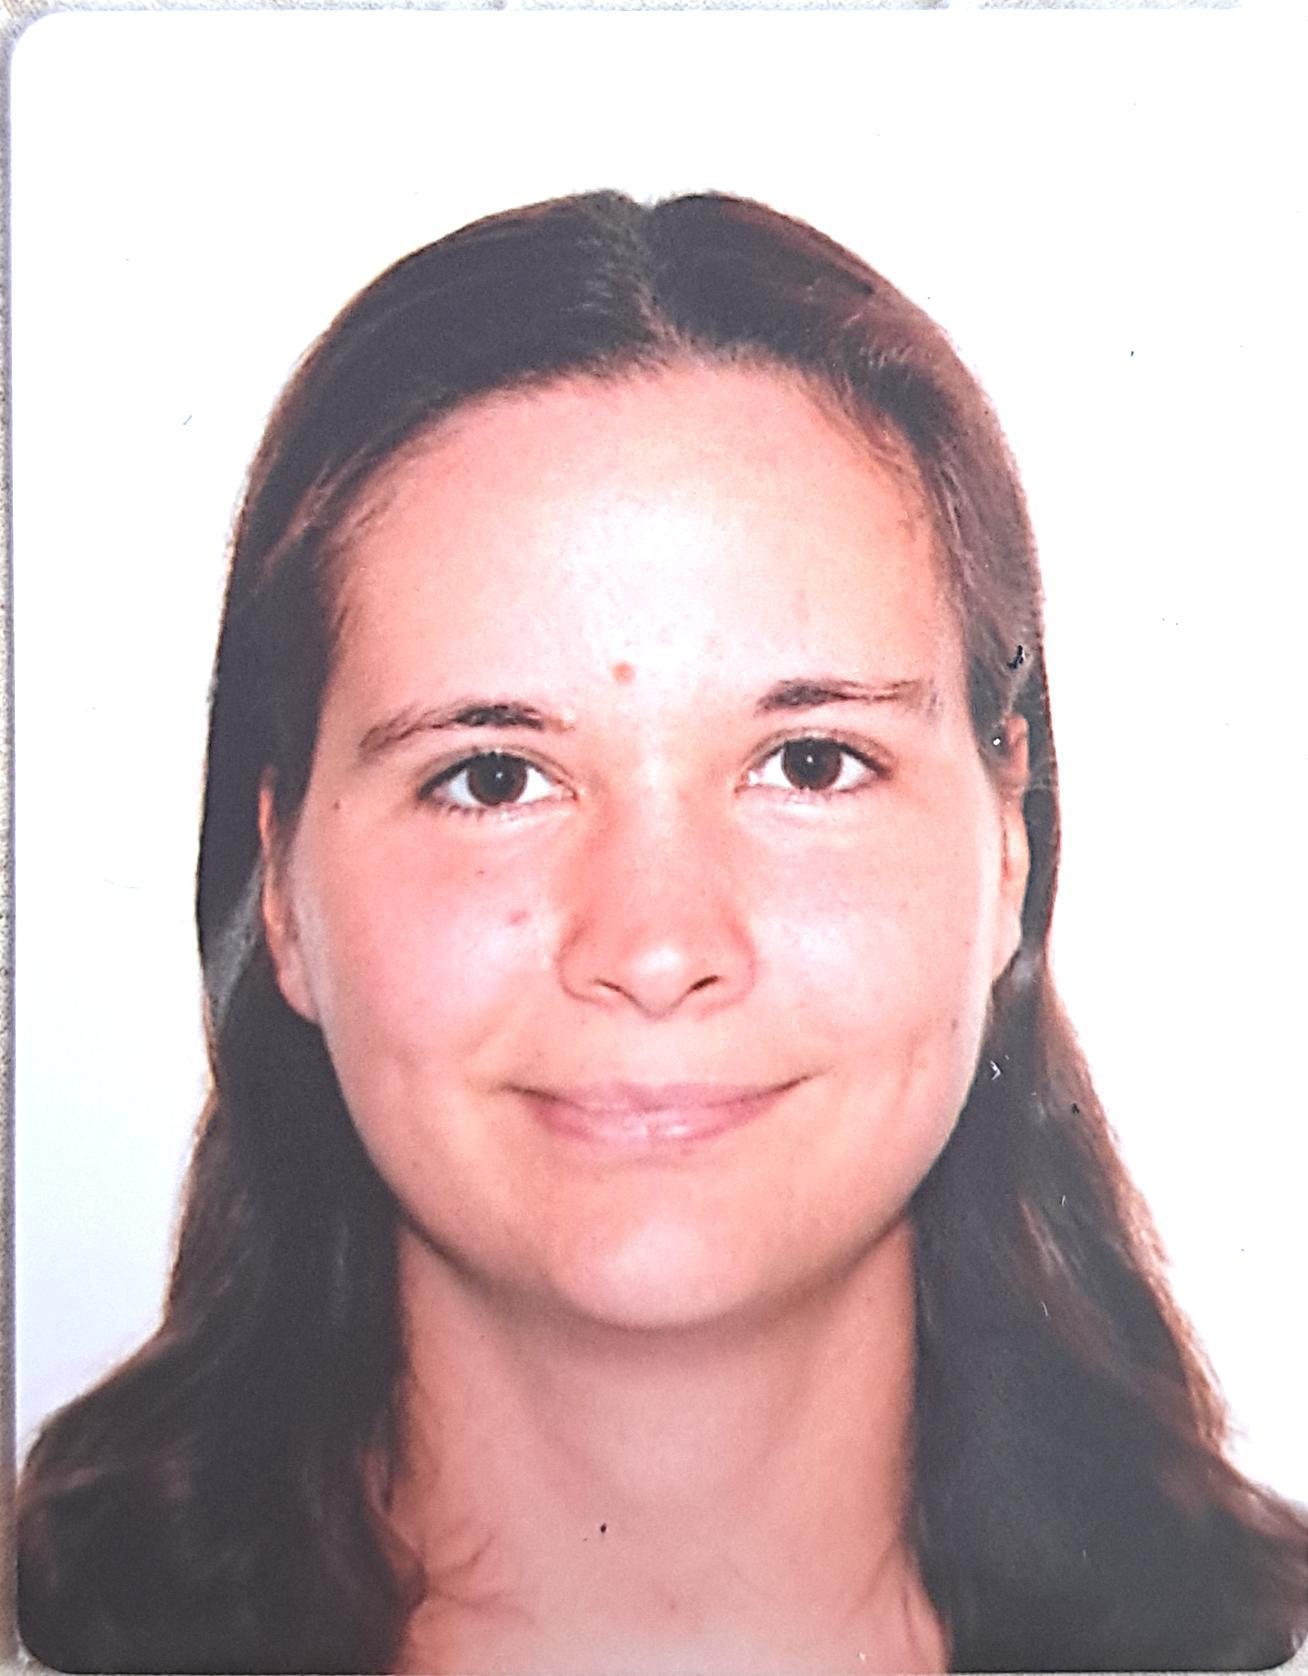
\includegraphics[width=\linewidth]{img/Borbala_Merth.jpg}
    \end{tabular}

\subsection{Márton Petes}
    \begin{tabular}{@{}p{0.7\textwidth}@{} p{0.3\textwidth}@{}}
    Test engineer and software engineer
    
    Main tasks:
    \begin{itemize}
        \item Testing the program
        \item Implementation in Model layer
    \end{itemize}
    &
    
\includegraphics[width=\linewidth]{img/Marton_Petes.png}
    \end{tabular}

\subsection{Dániel Gergely}
    \begin{tabular}{@{}p{0.7\textwidth}@{} p{0.2\textwidth}@{}}
    Full stack developer
    
    Main tasks:
    \begin{itemize}
        \item Implementation in Persistence layer
        \item GUI implementation
    \end{itemize}
    &
    
\includegraphics[width=\linewidth]{img/Daniel_Gergely.jpg}
    \end{tabular}

\subsection{Benedek Csüllög}
    \begin{tabular}{@{}p{0.7\textwidth}@{} p{0.2\textwidth}@{}}
    Software engineer and architect
    
    Main tasks:
    \begin{itemize}
        \item Architecture of the program
        \item Implementation in Model layer
    \end{itemize}
    &
    
\includegraphics[width=\linewidth]{img/Benedek_Csullog.jpg}
    \end{tabular}

\section{Completed MVP parts}

\begin{figure}[h]
    \centering
    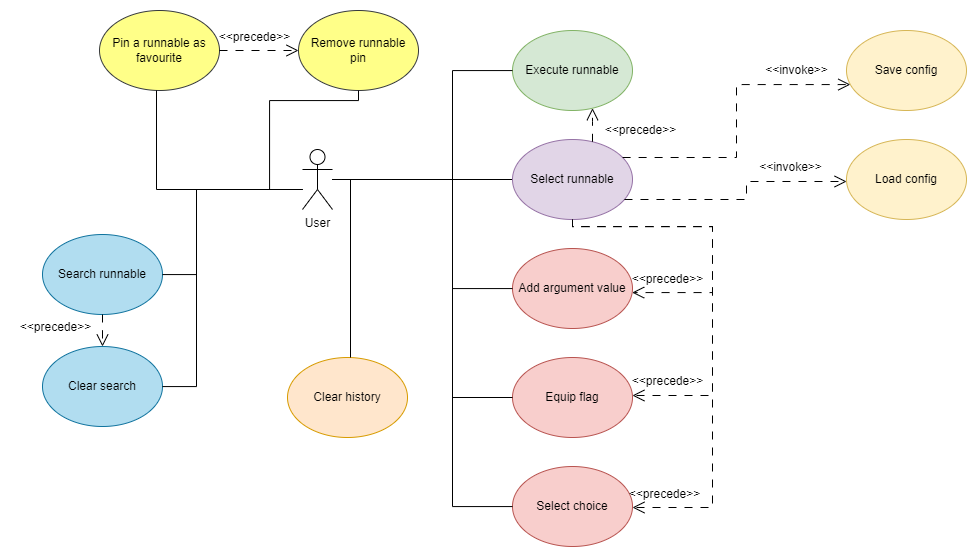
\includegraphics[width=1\linewidth]{img/use_case_diagram.drawio.png}
    \caption{Use case diagram}
    \label{fig:enter-label}
\end{figure}

\subsection{Content of the MVP}
Here are the \href{https://github.com/CsullogBeni/szofttech/blob/main/documentation/mvp.pdf}{MVP} points that we have fulfilled:
\begin{itemize}
    \item Select executable
    \item Add values to arguments
    \item Toggle flag
    \item Select choices
    \item Execute program
    \item Save config
    \item Load config
    \item Clear history
    \item Search executable
    \item Clear search
    \item Pin an executable
    \item Unpin an executable
\end{itemize}

\subsection{MVP parts in the program}

After the program initialization, on the main page:
\begin{itemize}
    \item The Users are able to set the current working directory.
    \item Users are also able to set their configuration history.
    \item The Users can search for their executable scripts from the working directory.
    \item They can also clear their search.
    \item On the main page all the pinned executable files are shown first.
    \item After the pinned ones, there are all the other scripts.
    \item Next to the executable button the Users can set the pinned status of a script.
\end{itemize}

\begin{figure}[h]
    \centering
    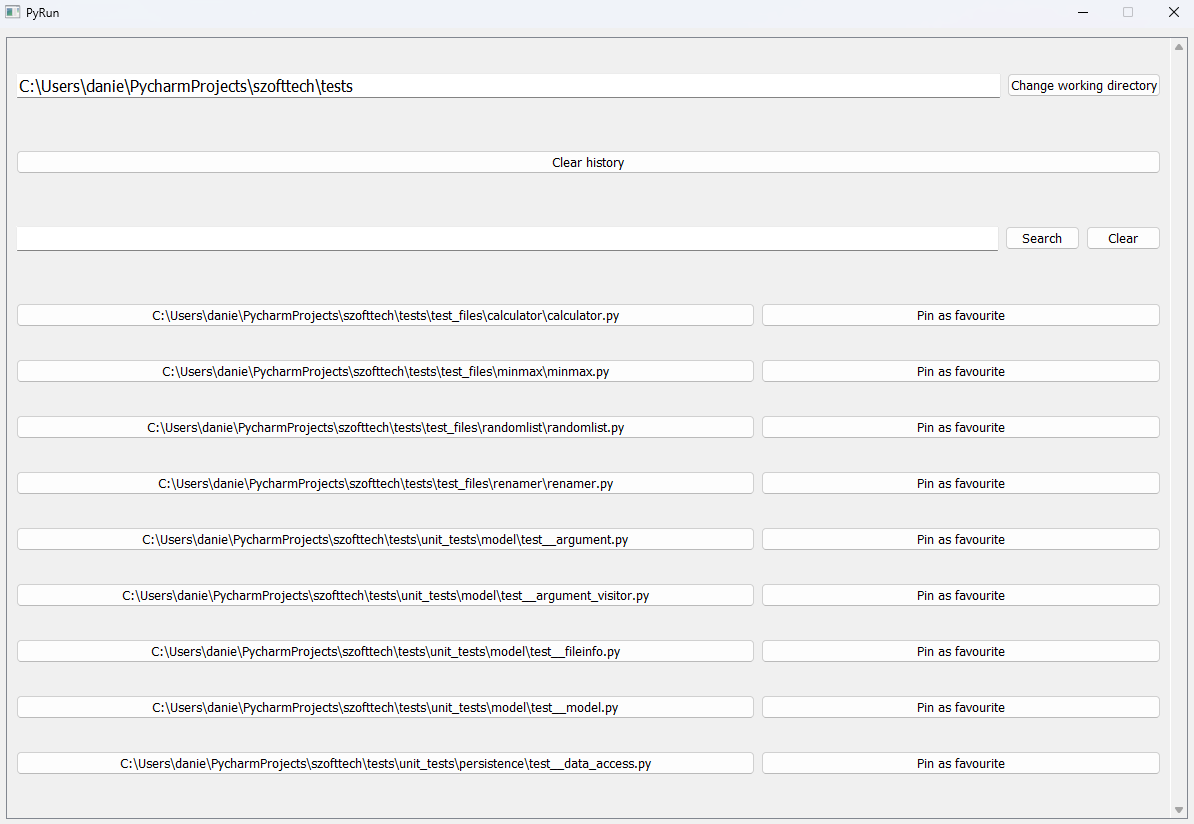
\includegraphics[width=1\linewidth]{img/main_page.png}
    \caption{Main page}
    \label{fig:enter-label}
\end{figure}

\begin{figure}[h]
    \centering
    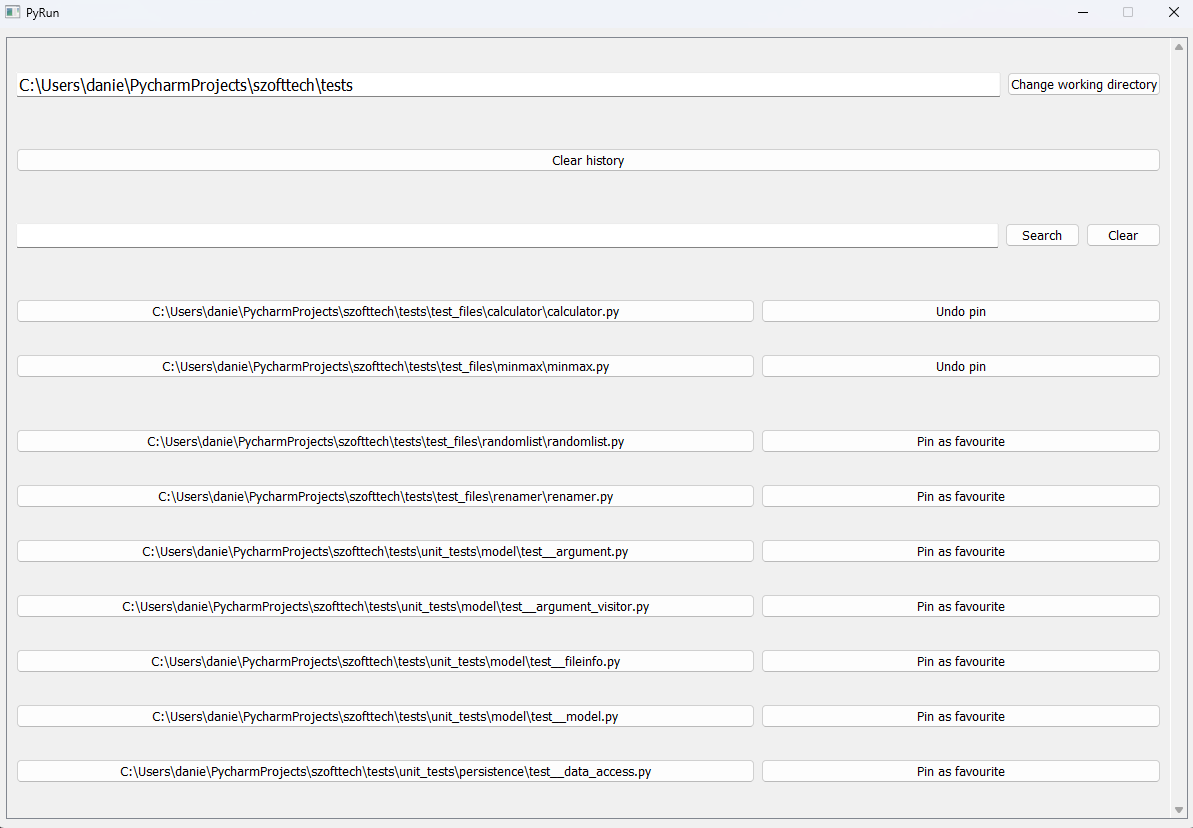
\includegraphics[width=1\linewidth]{img/pinned.png}
    \caption{Main page with pinned runnable}
    \label{fig:enter-label}
\end{figure}


\begin{figure}[h]
    \centering
    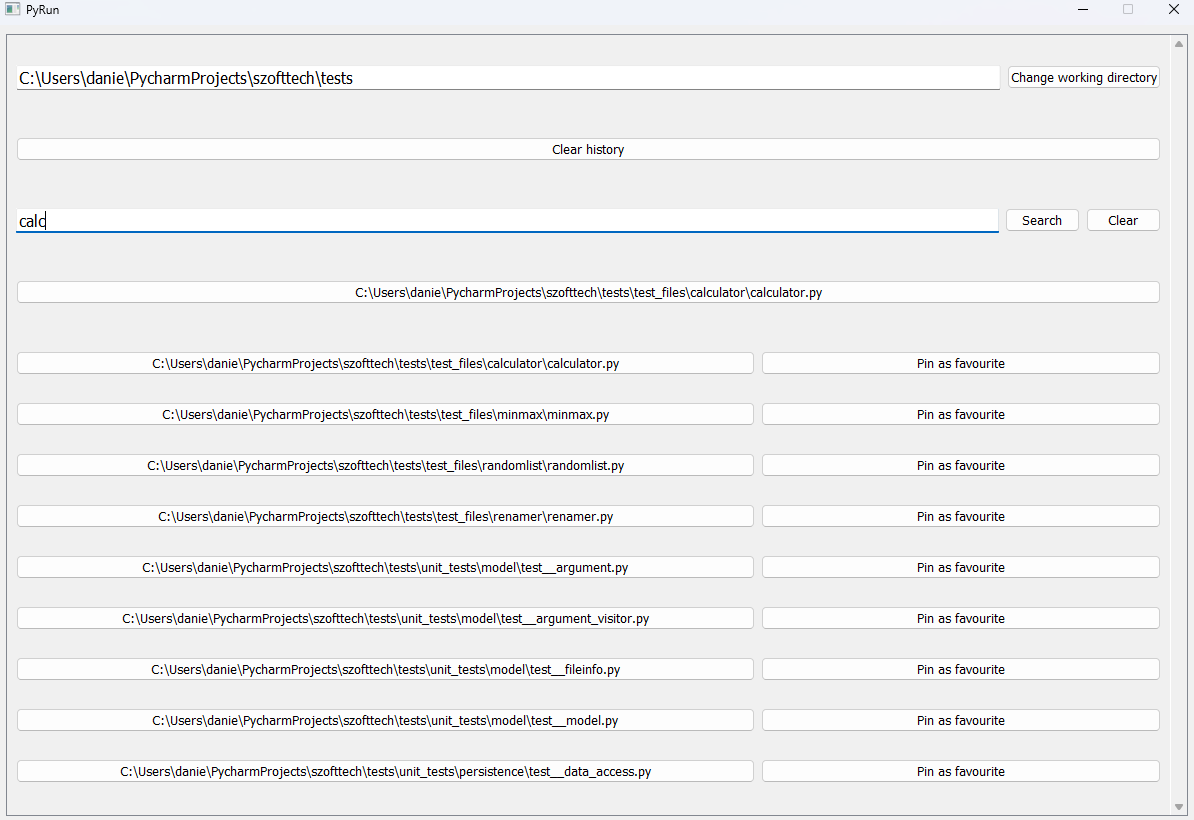
\includegraphics[width=1\linewidth]{img/search.png}
    \caption{Main page when the User searches}
    \label{fig:enter-label}
\end{figure}

\clearpage

After the User clicks on an executable, on the configuration page:
\begin{itemize}
    \item The Users can see every important information about the executable.
    \item The Users are able to add values to the arguments in an input field. 
    \item They can toggle flag arguments of the executable.
    \item If the argument contains choices, the program offers these choices in a list format, and the Users can select from the given list.
    \item The program saves the last configuration automatically and if the same configuration page is opened again, the program loads the last argument configuration.
    \item One of the main feature of the program is that the Users can execute the scripts directly from the tool.
    \item Last but not least, the Users can clear the current configuration.
\end{itemize}

\begin{figure}[h]
    \centering
    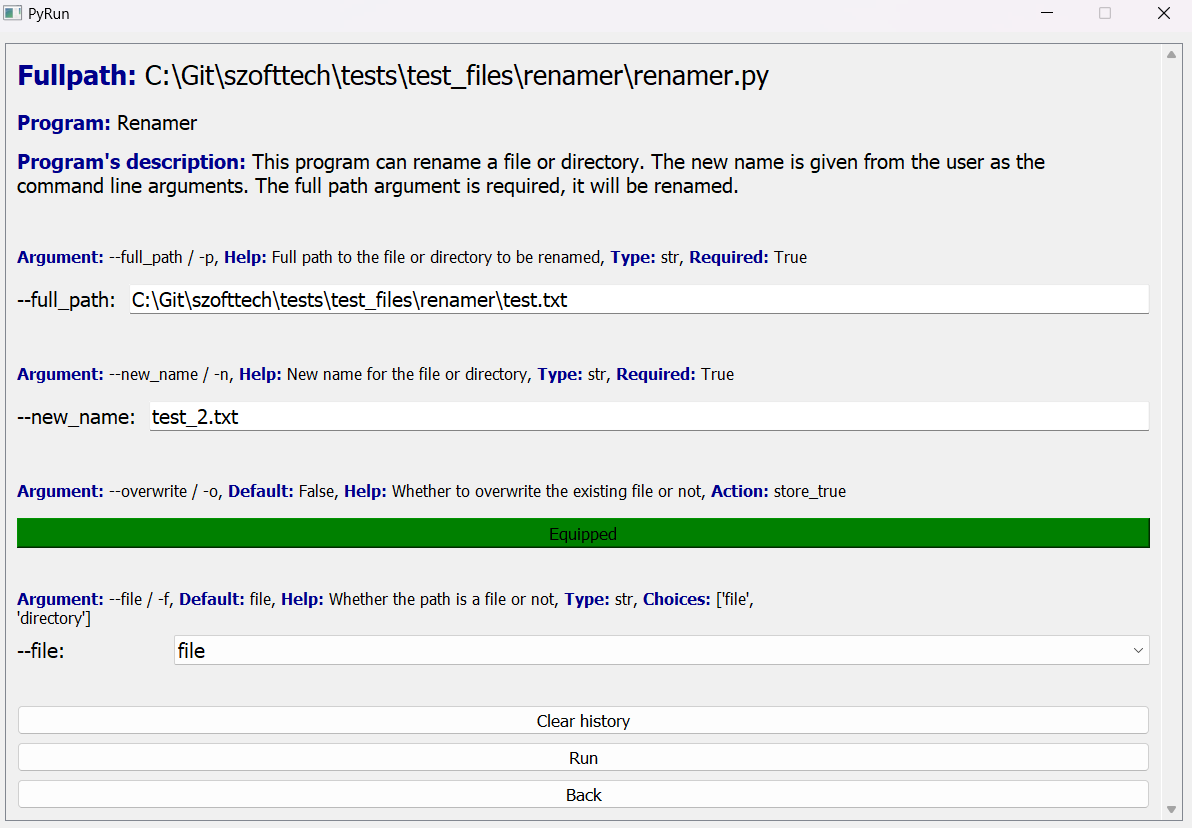
\includegraphics[width=1\linewidth]{img/config_page.png}
    \caption{Configuration page}
    \label{fig:enter-label}
\end{figure}

\clearpage

After running a script the Users are able to see the output of a program, or the error message if something goes wrong.

\begin{figure}[h]
    \centering
    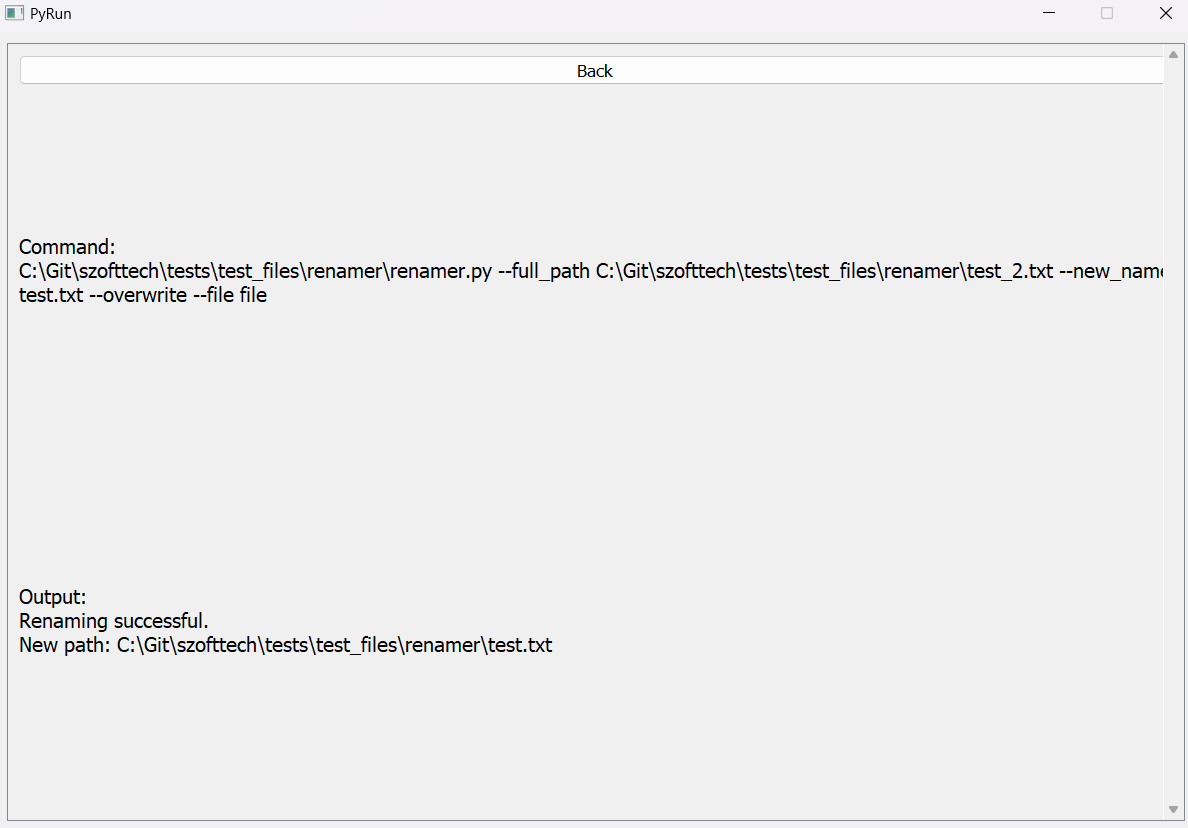
\includegraphics[width=1\linewidth]{img/runner_page.png}
    \caption{Runner page}
    \label{fig:enter-label}
\end{figure}

\subsection{Conclusion}

We are pleased to confirm that all the MVP features outlined above have been successfully implemented in the program. Each point has been carefully developed and integrated, ensuring the application meets the initial goals and requirements.

In conclusion, we have tried to create a program that simplifies developers’ lives by addressing common challenges and streamlining their workflow. While the program already offers valuable features, it holds significant potential for further development. Enhancements could make it even more universal, enabling it to cater to a broader range of needs and Users. By continuing to refine and expand its capabilities, the program could become an indispensable tool for developers worldwide.

\subsection{Ideas for the future}

Points that are not in the MVP, but in future iterations can be new features:
    \begin{itemize}
        \item .exe for the program - easier program start
        \item Our software could potentially recognize, analyze, and execute executable scripts written in multiple different programming languages. Each new programming language would be an extension of the product.
    \end{itemize}

\clearpage

\section{User Statistics}
The completed software was tested by our IT colleagues. The goal was to assess the program's functionality, usability, and performance in real-world scenarios.

\subsection{Participant Demographics}
Number of Participants: 5\\
Professional Background: All participants have an IT or software development background. \\
Roles Involved:
\begin{itemize}
    \item DevOps Engineer: 1
    \item Front-end Developer: 1
    \item Back-end Developer: 1
    \item Full-stack Developer: 1
    \item System Administrators: 1
\end{itemize}

\subsection{Methodology}
Duration: Each participant tested the program for approximately 2 hours. \\
Environment: Testing was conducted on individual workstations with different hardware and software configurations. \\
Test Scenarios: Participants were asked to perform the following tasks:
\begin{enumerate}
    \item Load predefined scripts.
    \item Handle the loaded scripts (search, pin as favourite).
    \item Configure different arguments of the scripts.
    \item Execute scripts.
    \item View the outputs after successful and unsuccessful runs.
\end{enumerate}

\subsection{Key Metrics Collected}
Task Completion Rate: \\
Most participants successfully completed all assigned tasks within the given time frame.
\begin{itemize}
    \item Overall: 100\%
    \item Loading and Executing Scripts: 98\%
    \item Error Handling and Log Viewing: 96\%
\end{itemize}

\noindent Average Task Completion Time:
\begin{itemize}
    \item Loading and handling scripts: 5 minutes
    \item Execute scripts: 15 minutes
    \item Analyse outputs 8 minutes
\end{itemize}

\noindent Error Rate: 5\%, common issues identified:
\begin{itemize}
    \item Script syntax validation: 30\%
    \item Display of outputs: 20\%
    \item External dependency management: 45\%
    \item Other: 5\%
\end{itemize}

\noindent Performance Metrics:
\begin{itemize}
    \item Script Execution Success Rate: 98\%
    \item Average Script Execution Time:
    \begin{itemize}
        \item Small scripts (<100 lines): 1.5 seconds
        \item Medium scripts (100-500 lines): 3.2 seconds
        \item Large scripts (>500 lines): 7.8 seconds
    \end{itemize}
    \item Peak Memory Usage: our program has low memory usage, so it depends on the scripts
\end{itemize}


\subsection{User Feedback Summary}
\begin{itemize}
    \item Ease of Use:\\
    95\% of participants found the GUI intuitive and user-friendly. Suggested improvements included adding tooltips.
    \item Performance:\\
    The majority reported smooth performance. One participant noted a slight delay when handling lots of scripts.
    \item Functionality:\\
    We have got positive feedback on the implemented features.
    \item Stability:\\
    No crashes were reported during testing. Minor bugs were identified in the log display feature, which have been noted for fixing.
\end{itemize}

\section{KPI goals}
We have defined the KPI this way: \\
The KPI measures the completion rate of the core features and functionalities planned for the project.
This metric helped us objectively assess the progress and success of the project by focusing on the implementation of key deliverables that form the foundation of the system's functionality. \\
The KPI is calculated as the percentage of core features implemented out of the total planned features. In our case, these core features were clearly defined and broken down into 12 specific use cases, each representing a critical aspect of the project's functionality. These use cases were identified during the planning phase, with careful consideration of both stakeholder requirements and technical feasibility, ensuring that they accurately reflect the project's objectives. \\
At the conclusion of the implementation phase, we verified that all 12 planned use cases had been successfully developed. Therefore our KPI can be calculated as follows:
\[ \frac{implemented\ use\ cases}{planned\ use\ cases} * 100 = \frac{12}{12}*100 = 100 \]

As a result, our KPI is 100\%, and since our target was also to achieve 100\%, we can confidently state that we have successfully completed our goal. This accomplishment is a testament to the team's hard work, effective planning, and strong collaboration throughout the projects lifecycle.

\end{document}